\documentclass{beamer}
\usepackage[utf8]{inputenc}

\usetheme{Madrid}
\usecolortheme{default}
\usepackage{amsmath,amssymb,amsfonts,amsthm}
\usepackage{txfonts}
\usepackage{tkz-euclide}
\usepackage{listings}
\usepackage{adjustbox}
\usepackage{array}
\usepackage{tabularx}
\usepackage{gvv}
\usepackage{lmodern}
\usepackage{circuitikz}
\usepackage{tikz}
\usepackage{graphicx}

\setbeamertemplate{page number in head/foot}[totalframenumber]

\usepackage{tcolorbox}
\tcbuselibrary{minted,breakable,xparse,skins}
\documentclass{beamer}
\usepackage[utf8]{inputenc}

\usetheme{Madrid}
\usecolortheme{default}
\usepackage{amsmath,amssymb,amsfonts,amsthm}
\usepackage{txfonts}
\usepackage{tkz-euclide}
\usepackage{listings}
\usepackage{adjustbox}
\usepackage{array}
\usepackage{tabularx}
\usepackage{gvv}
\usepackage{lmodern}
\usepackage{circuitikz}
\usepackage{tikz}
\usepackage{graphicx}

\setbeamertemplate{page number in head/foot}[totalframenumber]

\usepackage{tcolorbox}
\tcbuselibrary{minted,breakable,xparse,skins}



\definecolor{bg}{gray}{0.95}
\DeclareTCBListing{mintedbox}{O{}m!O{}}{%
  breakable=true,
  listing engine=minted,
  listing only,
  minted language=#2,
  minted style=default,
  minted options={%
    linenos,
    gobble=0,
    breaklines=true,
    breakafter=,,
    fontsize=\small,
    numbersep=8pt,
    #1},
  boxsep=0pt,
  left skip=0pt,
  right skip=0pt,
  left=25pt,
  right=0pt,
  top=3pt,
  bottom=3pt,
  arc=5pt,
  leftrule=0pt,
  rightrule=0pt,
  bottomrule=2pt,
  toprule=2pt,
  colback=bg,
  colframe=orange!70,
  enhanced,
  overlay={%
    \begin{tcbclipinterior}
    \fill[orange!20!white] (frame.south west) rectangle ([xshift=20pt]frame.north west);
    \end{tcbclipinterior}},
  #3,
}
\lstset{
    language=C,
    basicstyle=\ttfamily\small,
    keywordstyle=\color{blue},
    stringstyle=\color{orange},
    commentstyle=\color{green!60!black},
    numbers=left,
    numberstyle=\tiny\color{gray},
    breaklines=true,
    showstringspaces=false,
}
%------------------------------------------------------------
%This block of code defines the information to appear in the
%Title page
\title %optional
{1.5.1}
\date{August 22,2025}
%\subtitle{A short story}

\author % (optional)
{Bhargav - EE25BTECH11013}



\begin{document}


\frame{\titlepage}
\begin{frame}{Question}
The center of a circle whose endpoints of a diameter of the circle A, B are \brak{-6,3} and \brak{6,4} is\\
\end{frame}



\begin{frame}{Theoretical Solution}

Let the endpoints of the diameter of the circle be $\vec{A}$ and $\vec{B}$:
\begin{align}
    \vec{A}=\begin{myvec}{-6\\3}\end{myvec} \;, \vec{B}=\begin{myvec}{6\\4} \end{myvec}
\end{align}

We can use the midpoint formula to find the center of the circle.\\

\end{frame}

\begin{frame}{Equation}
\textbf{Midpoint $\vec{C}$ of the vectors $\vec{A}$ and $\vec{B}$ is given by}
\begin{align}
    \vec{C}=\frac{\vec{A}+\vec{B}}{2} 
\end{align}
\end{frame}
\begin{frame}{Equation}

\begin{align}
    \vec{C}=\frac{1}{2}\myvec{-6+6 \\ 3+4} 
\end{align}
\begin{align}
    \vec{C}=\frac{1}{2} \myvec{0 \\ 7} 
\end{align}
\begin{align}
    \vec{C}=\myvec{0\\\tfrac{7}{2}}.
\end{align}
\end{frame}

\begin{frame}[fragile]
    \frametitle{C Code - Midpoint formula}

    \begin{lstlisting}

#include <stdio.h>

void midpt(double x1, double y1, double x2, double y2, double* x, double* y) {
    *x = (x2 + x1) / (2);
    *y = (y2 + y1) / (2);
}

    \end{lstlisting}
\end{frame}

\begin{frame}[fragile]
    \frametitle{Python + C Code}
    \begin{lstlisting}
import ctypes
import numpy as np
import matplotlib.pyplot as plt

# Load shared object
lib = ctypes.CDLL("./libmidpt.so")

# Define C function prototype
lib.midpt.argtypes = [ctypes.c_double, ctypes.c_double,
                      ctypes.c_double, ctypes.c_double,
                      ctypes.POINTER(ctypes.c_double), ctypes.POINTER(ctypes.c_double)]

# Input diameter endpoints
x1, y1 = -6.0, 3.0
x2, y2 = 6.0, 4.0

    \end{lstlisting}
\end{frame}

\begin{frame}[fragile]
    \frametitle{Python + C Code}
    \begin{lstlisting}
# Prepare output variables
x_mid = ctypes.c_double()
y_mid = ctypes.c_double()

# Call C function
lib.midpt(x1, y1, x2, y2, ctypes.byref(x_mid), ctypes.byref(y_mid))

cx, cy = x_mid.value, y_mid.value
print("Centre of circle:", (cx, cy))

# Radius = half distance between endpoints
r = np.sqrt((x2 - x1)**2 + (y2 - y1)**2) / 2

# Generate circle points
theta = np.linspace(0, 2*np.pi, 500)
x_circle = cx + r * np.cos(theta)
y_circle = cy + r * np.sin(theta)

    \end{lstlisting}
\end{frame}

\begin{frame}[fragile]
    \frametitle{Python + C Code}
    \begin{lstlisting}
# Plot
plt.figure(figsize=(6,6))
plt.plot(x_circle, y_circle, label="Circle")
plt.scatter([x1, x2], [y1, y2], color="red", s=80, label="Diameter Endpoints")
plt.text(x1 - 1, y1 - 0.5, f"({x1:.0f}, {y1:.0f})", color="red", fontsize=10)
plt.text(x2 + 0.5, y2, f"({x2:.0f}, {y2:.0f})", color="red", fontsize=10)

plt.scatter(cx, cy, color="blue", marker="x", s=200, linewidths=3, label="Centre")
plt.text(cx + 0.5, cy + 0.5, f"({cx:.2f}, {cy:.2f})", color="blue", fontsize=10)
plt.plot([x1, x2], [y1, y2], 'g--', label="Diameter")

    \end{lstlisting}
\end{frame}


\begin{frame}[fragile]
    \frametitle{Python + C Code}
    \begin{lstlisting}
plt.axis("equal")
plt.legend(loc="upper right")
plt.title("Circle from Diameter Endpoints")
plt.savefig("/Users/bhargavkrish/Documents/ee1030-2025/ee25btech11013/matgeo/1.5.1/figs/Figure_1.png")
plt.show()
    \end{lstlisting}
\end{frame}

\begin{frame}[fragile]
    \frametitle{Python Code}
    \begin{lstlisting}
import numpy as np
import matplotlib.pyplot as plt

# Input diameter endpoints
x1, y1 = -6.0, 3.0
x2, y2 = 6.0, 4.0

# Midpoint (centre of circle)
cx = (x1 + x2) / 2
cy = (y1 + y2) / 2
print("Centre of circle:", (cx, cy))

# Radius = half distance between endpoints
r = np.sqrt((x2 - x1)**2 + (y2 - y1)**2) / 2


    \end{lstlisting}
\end{frame}

\begin{frame}[fragile]
    \frametitle{Python Code}
    \begin{lstlisting}

# Generate circle points
theta = np.linspace(0, 2*np.pi, 500)
x_circle = cx + r * np.cos(theta)
y_circle = cy + r * np.sin(theta)

# Plot
plt.figure(figsize=(6,6))
plt.plot(x_circle, y_circle, label="Circle")

plt.scatter([x1, x2], [y1, y2], color="red", s=80, label="Diameter Endpoints")
plt.text(x1 - 1, y1 - 0.5, f"({x1:.0f}, {y1:.0f})", color="red", fontsize=10)
plt.text(x2 + 0.5, y2, f"({x2:.0f}, {y2:.0f})", color="red", fontsize=10)

    \end{lstlisting}
\end{frame}

\begin{frame}[fragile]
    \frametitle{Python Code}
    \begin{lstlisting}
plt.scatter(cx, cy, color="blue", marker="x", s=200, linewidths=3, label="Centre")
plt.text(cx + 0.5, cy + 0.5, f"({cx:.2f}, {cy:.2f})", color="blue", fontsize=10)

plt.plot([x1, x2], [y1, y2], 'g--', label="Diameter")
plt.axis("equal")
plt.legend(loc="upper right")
plt.title("Circle from Diameter Endpoints")
plt.savefig("/Users/bhargavkrish/Documents/ee1030-2025/ee25btech11013/matgeo/1.5.1/figs/Figure_1.png")
plt.show()
    \end{lstlisting}
\end{frame}

\begin{frame}{Plot}
    \centering
    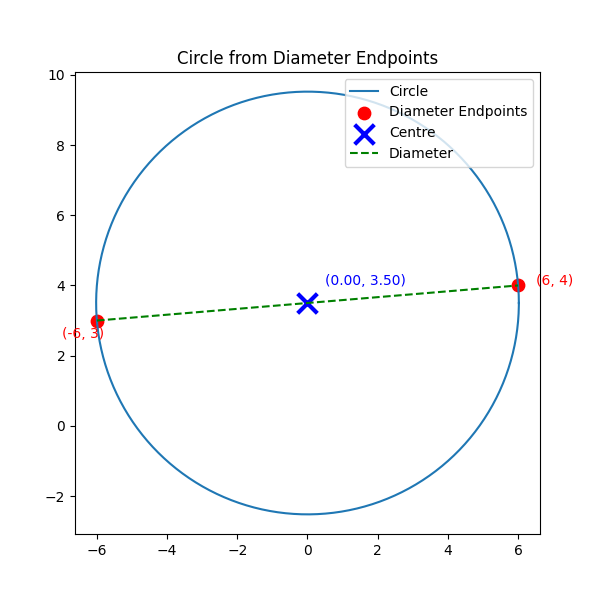
\includegraphics[width=3\columnwidth, height=0.8\textheight, keepaspectratio]{figs/Figure_1.png}     
\end{frame}


\end{document}


\definecolor{bg}{gray}{0.95}
\DeclareTCBListing{mintedbox}{O{}m!O{}}{%
  breakable=true,
  listing engine=minted,
  listing only,
  minted language=#2,
  minted style=default,
  minted options={%
    linenos,
    gobble=0,
    breaklines=true,
    breakafter=,,
    fontsize=\small,
    numbersep=8pt,
    #1},
  boxsep=0pt,
  left skip=0pt,
  right skip=0pt,
  left=25pt,
  right=0pt,
  top=3pt,
  bottom=3pt,
  arc=5pt,
  leftrule=0pt,
  rightrule=0pt,
  bottomrule=2pt,
  toprule=2pt,
  colback=bg,
  colframe=orange!70,
  enhanced,
  overlay={%
    \begin{tcbclipinterior}
    \fill[orange!20!white] (frame.south west) rectangle ([xshift=20pt]frame.north west);
    \end{tcbclipinterior}},
  #3,
}
\lstset{
    language=C,
    basicstyle=\ttfamily\small,
    keywordstyle=\color{blue},
    stringstyle=\color{orange},
    commentstyle=\color{green!60!black},
    numbers=left,
    numberstyle=\tiny\color{gray},
    breaklines=true,
    showstringspaces=false,
}
%------------------------------------------------------------
%This block of code defines the information to appear in the
%Title page
\title %optional
{1.5.1}
\date{August 22,2025}
%\subtitle{A short story}

\author % (optional)
{Bhargav - EE25BTECH11013}



\begin{document}


\frame{\titlepage}
\begin{frame}{Question}
The center of a circle whose endpoints of a diameter of the circle A, B are \brak{-6,3} and \brak{6,4} is\\
\end{frame}



\begin{frame}{Theoretical Solution}

Let the endpoints of the diameter of the circle be $\vec{A}$ and $\vec{B}$:
\begin{align}
    \vec{A}=\begin{myvec}{-6\\3}\end{myvec} \;, \vec{B}=\begin{myvec}{6\\4} \end{myvec}
\end{align}

We can use the midpoint formula to find the center of the circle.\\

\end{frame}

\begin{frame}{Equation}
\textbf{Midpoint $\vec{C}$ of the vectors $\vec{A}$ and $\vec{B}$ is given by}
\begin{align}
    \vec{C}=\frac{\vec{A}+\vec{B}}{2} 
\end{align}
\end{frame}
\begin{frame}{Equation}

\begin{align}
    \vec{C}=\frac{1}{2}\myvec{-6+6 \\ 3+4} 
\end{align}
\begin{align}
    \vec{C}=\frac{1}{2} \myvec{0 \\ 7} 
\end{align}
\begin{align}
    \vec{C}=\myvec{0\\\tfrac{7}{2}}.
\end{align}
\end{frame}

\begin{frame}[fragile]
    \frametitle{C Code - Midpoint formula}

    \begin{lstlisting}

#include <stdio.h>

void midpt(double x1, double y1, double x2, double y2, double* x, double* y) {
    *x = (x2 + x1) / (2);
    *y = (y2 + y1) / (2);
}

    \end{lstlisting}
\end{frame}

\begin{frame}[fragile]
    \frametitle{Python Code}
    \begin{lstlisting}
import ctypes
import numpy as np
import matplotlib.pyplot as plt

# Load shared object
lib = ctypes.CDLL("./libmidpt.so")

# Define C function prototype
lib.midpt.argtypes = [ctypes.c_double, ctypes.c_double,
                      ctypes.c_double, ctypes.c_double,
                      ctypes.POINTER(ctypes.c_double), ctypes.POINTER(ctypes.c_double)]

# Input diameter endpoints
x1, y1 = -6.0, 3.0
x2, y2 = 6.0, 4.0

    \end{lstlisting}
\end{frame}

\begin{frame}[fragile]
    \frametitle{Python Code}
    \begin{lstlisting}
# Prepare output variables
x_mid = ctypes.c_double()
y_mid = ctypes.c_double()

# Call C function
lib.midpt(x1, y1, x2, y2, ctypes.byref(x_mid), ctypes.byref(y_mid))

cx, cy = x_mid.value, y_mid.value
print("Centre of circle:", (cx, cy))

# Radius = half distance between endpoints
r = np.sqrt((x2 - x1)**2 + (y2 - y1)**2) / 2

# Generate circle points
theta = np.linspace(0, 2*np.pi, 500)
x_circle = cx + r * np.cos(theta)
y_circle = cy + r * np.sin(theta)

    \end{lstlisting}
\end{frame}

\begin{frame}[fragile]
    \frametitle{Python Code}
    \begin{lstlisting}
# Plot
plt.figure(figsize=(6,6))
plt.plot(x_circle, y_circle, label="Circle")
plt.scatter([x1, x2], [y1, y2], color="red", s=80, label="Diameter Endpoints")
plt.text(x1 - 1, y1 - 0.5, f"({x1:.0f}, {y1:.0f})", color="red", fontsize=10)
plt.text(x2 + 0.5, y2, f"({x2:.0f}, {y2:.0f})", color="red", fontsize=10)

plt.scatter(cx, cy, color="blue", marker="x", s=200, linewidths=3, label="Centre")
plt.text(cx + 0.5, cy + 0.5, f"({cx:.2f}, {cy:.2f})", color="blue", fontsize=10)
plt.plot([x1, x2], [y1, y2], 'g--', label="Diameter")

    \end{lstlisting}
\end{frame}


\begin{frame}[fragile]
    \frametitle{Python Code}
    \begin{lstlisting}
plt.axis("equal")
plt.legend(loc="upper right")
plt.title("Circle from Diameter Endpoints")
plt.savefig("/Users/bhargavkrish/Documents/ee1030-2025/ee25btech11013/matgeo/1.5.1/figs/Figure_1.png")
plt.show()
    \end{lstlisting}
\end{frame}


\begin{frame}{Plot}
    \centering
    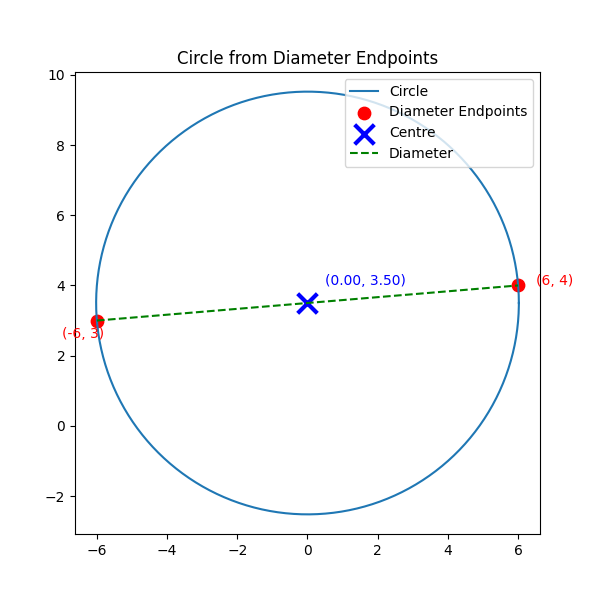
\includegraphics[width=3\columnwidth, height=0.8\textheight, keepaspectratio]{figs/Figure_1.png}     
\end{frame}


\end{document}
